\documentclass[tikz,border=12pt]{standalone}
\usepackage[T1]{fontenc}
\usepackage{tgheros}
\usepackage{sfmath}
\usepackage{amsmath}
\usepackage{tikz}
\usetikzlibrary{arrows.meta,positioning,shapes.geometric,fit,backgrounds,calc}
\usepackage{xcolor}

\renewcommand{\familydefault}{\sfdefault}

% Academic Semantic Palette
\definecolor{harvardcrimson}{HTML}{A51C30}
\definecolor{ethdarkblue}{HTML}{1F407A}
\definecolor{ethblue}{HTML}{215CAF}
\definecolor{ethpetrol}{HTML}{007A87}
\definecolor{ethbronze}{HTML}{B87333}
\definecolor{ethpurple}{HTML}{5B4B8A}
\definecolor{ethslate}{HTML}{475569}
\definecolor{cardbg}{HTML}{F8FAFC}
\definecolor{cardborder}{HTML}{CBD5E1}
\definecolor{safeTeal}{HTML}{10B981}
\definecolor{amberProp}{HTML}{C98218}
\definecolor{amberBg}{HTML}{FFF3DC}
\definecolor{coralVeto}{HTML}{BD4F2F}
\definecolor{coralBg}{HTML}{FAE9E2}
\definecolor{navyBg}{HTML}{E8EDF6}
\definecolor{tealBg}{HTML}{E4F6F3}

\begin{document}
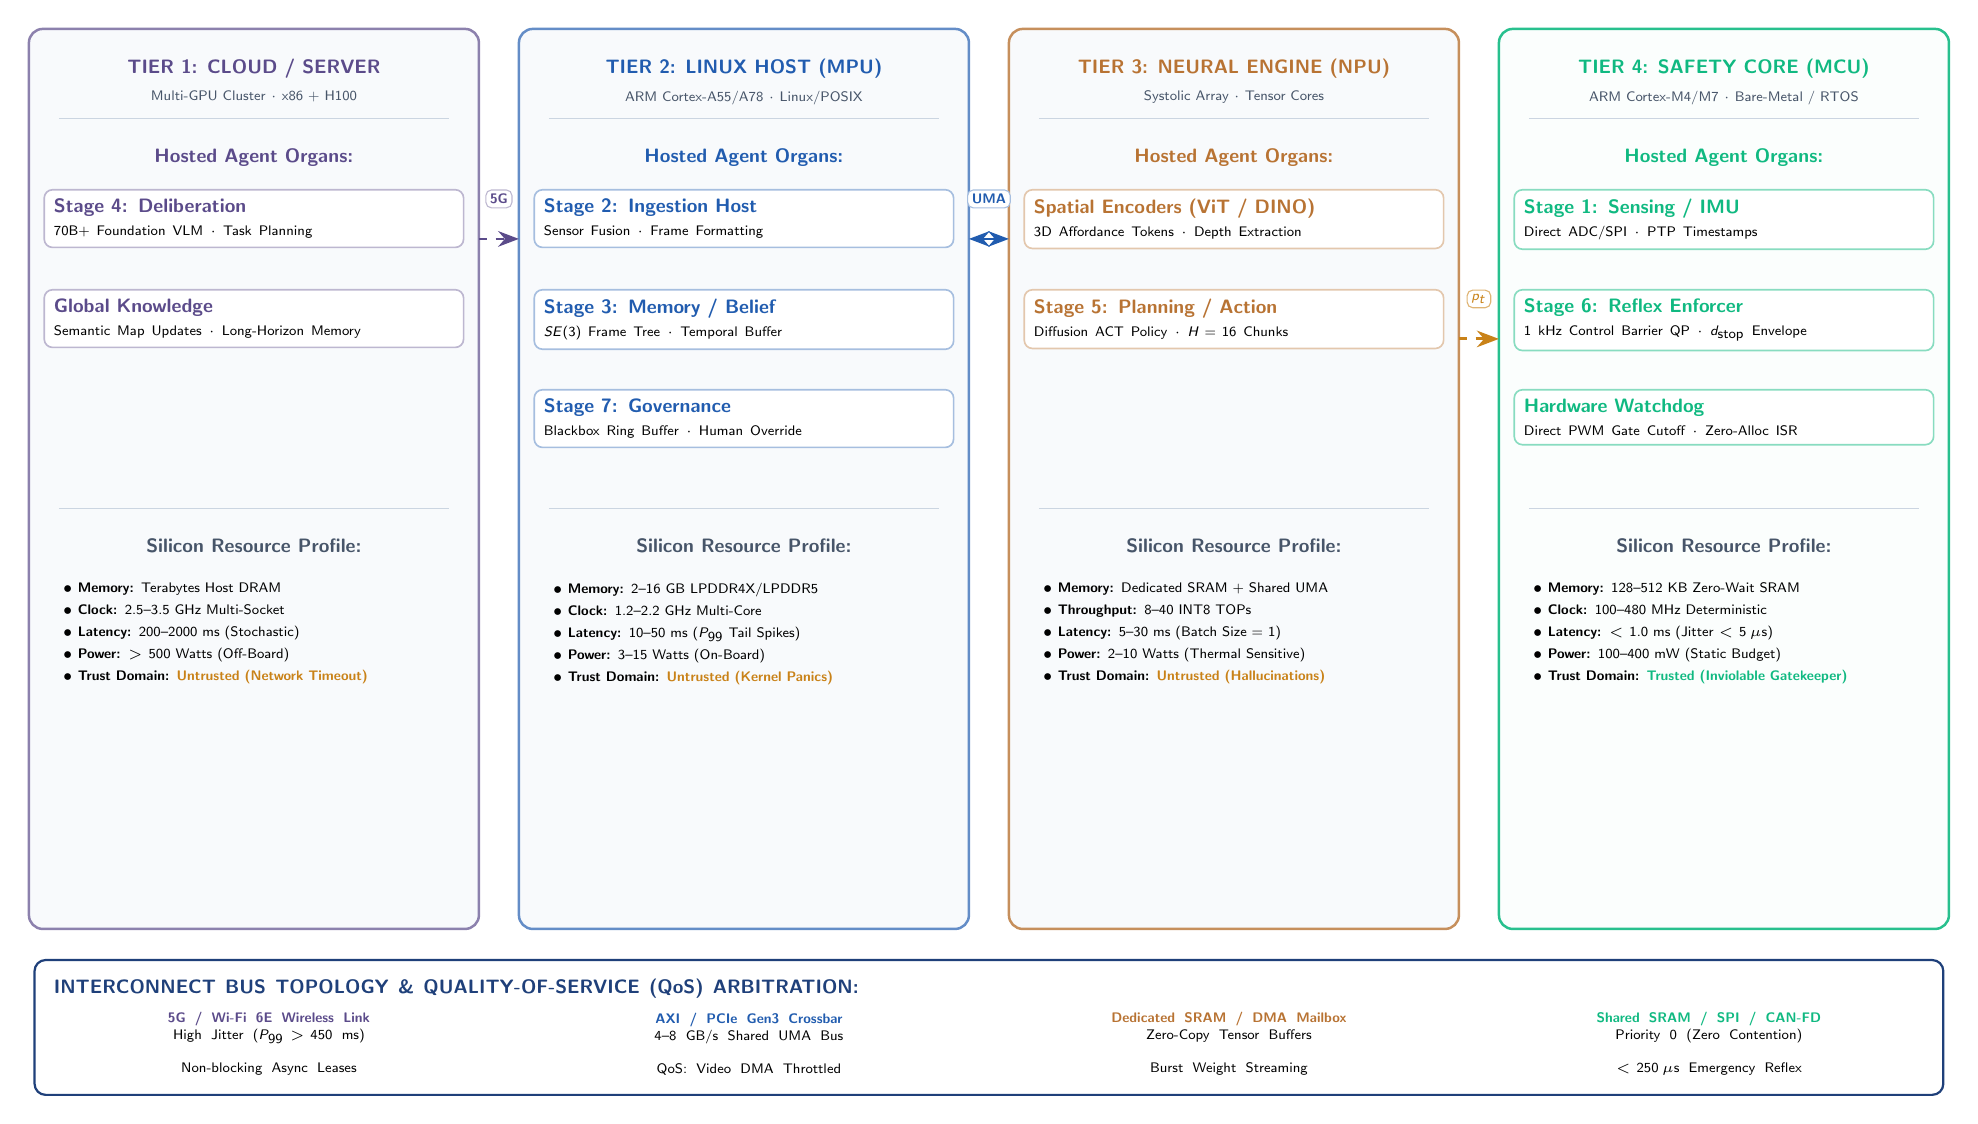
\begin{tikzpicture}[
  font=\sffamily,
  >=Stealth,
  stagepill/.style={
    draw=ethdarkblue!50,
    fill=white,
    rounded corners=3pt,
    line width=0.6pt,
    text width=2.00in,
    inner sep=3.5pt,
    align=left,
    font=\scriptsize
  }
]

  % ----------------------------------------------------
  % TIER 1: CLOUD / SERVER (x = 0 to 2.25in)
  % ----------------------------------------------------
  \draw[draw=ethpurple!70, fill=cardbg, rounded corners=5pt, line width=0.9pt]
    (0, 0) rectangle ++(2.25in, -4.50in);
  
  \node[anchor=north, font=\scriptsize\bfseries, color=ethpurple] at (1.125in, -0.10in) {TIER 1: CLOUD / SERVER};
  \node[anchor=north, font=\tiny, color=ethslate] at (1.125in, -0.26in) {Multi-GPU Cluster $\cdot$ x86 + H100};
  \draw[draw=cardborder, line width=0.4pt] (0.15in, -0.45in) -- (2.10in, -0.45in);

  \node[anchor=north, font=\scriptsize\bfseries, color=ethpurple] at (1.125in, -0.55in) {Hosted Agent Organs:};
  
  \node[stagepill, draw=ethpurple!40, anchor=north] at (1.125in, -0.80in) {
    \textbf{\color{ethpurple} Stage 4: Deliberation}\\
    {\tiny 70B+ Foundation VLM $\cdot$ Task Planning}
  };
  \node[stagepill, draw=ethpurple!40, anchor=north] at (1.125in, -1.30in) {
    \textbf{\color{ethpurple} Global Knowledge}\\
    {\tiny Semantic Map Updates $\cdot$ Long-Horizon Memory}
  };

  \draw[draw=cardborder, line width=0.4pt] (0.15in, -2.40in) -- (2.10in, -2.40in);
  \node[anchor=north, font=\scriptsize\bfseries, color=ethslate] at (1.125in, -2.50in) {Silicon Resource Profile:};
  \node[anchor=north west, font=\tiny, text width=2.00in, align=left] at (0.12in, -2.72in) {
    $\bullet$ \textbf{Memory:} Terabytes Host DRAM\\[2pt]
    $\bullet$ \textbf{Clock:} $2.5\text{--}3.5\text{ GHz}$ Multi-Socket\\[2pt]
    $\bullet$ \textbf{Latency:} $200\text{--}2000\text{ ms}$ (Stochastic)\\[2pt]
    $\bullet$ \textbf{Power:} $> 500\text{ Watts}$ (Off-Board)\\[2pt]
    $\bullet$ \textbf{Trust Domain:} \textbf{\color{amberProp}Untrusted (Network Timeout)}
  };

  % ----------------------------------------------------
  % TIER 2: LINUX HOST (MPU) (x = 2.45in to 4.70in)
  % ----------------------------------------------------
  \draw[draw=ethblue!70, fill=cardbg, rounded corners=5pt, line width=0.9pt]
    (2.45in, 0) rectangle ++(2.25in, -4.50in);
  
  \node[anchor=north, font=\scriptsize\bfseries, color=ethblue] at (3.575in, -0.10in) {TIER 2: LINUX HOST (MPU)};
  \node[anchor=north, font=\tiny, color=ethslate] at (3.575in, -0.26in) {ARM Cortex-A55/A78 $\cdot$ Linux/POSIX};
  \draw[draw=cardborder, line width=0.4pt] (2.60in, -0.45in) -- (4.55in, -0.45in);

  \node[anchor=north, font=\scriptsize\bfseries, color=ethblue] at (3.575in, -0.55in) {Hosted Agent Organs:};
  
  \node[stagepill, draw=ethblue!40, anchor=north] at (3.575in, -0.80in) {
    \textbf{\color{ethblue} Stage 2: Ingestion Host}\\
    {\tiny Sensor Fusion $\cdot$ Frame Formatting}
  };
  \node[stagepill, draw=ethblue!40, anchor=north] at (3.575in, -1.30in) {
    \textbf{\color{ethblue} Stage 3: Memory / Belief}\\
    {\tiny $SE(3)$ Frame Tree $\cdot$ Temporal Buffer}
  };
  \node[stagepill, draw=ethblue!40, anchor=north] at (3.575in, -1.80in) {
    \textbf{\color{ethblue} Stage 7: Governance}\\
    {\tiny Blackbox Ring Buffer $\cdot$ Human Override}
  };

  \draw[draw=cardborder, line width=0.4pt] (2.60in, -2.40in) -- (4.55in, -2.40in);
  \node[anchor=north, font=\scriptsize\bfseries, color=ethslate] at (3.575in, -2.50in) {Silicon Resource Profile:};
  \node[anchor=north west, font=\tiny, text width=2.00in, align=left] at (2.57in, -2.72in) {
    $\bullet$ \textbf{Memory:} $2\text{--}16\text{ GB}$ LPDDR4X/LPDDR5\\[2pt]
    $\bullet$ \textbf{Clock:} $1.2\text{--}2.2\text{ GHz}$ Multi-Core\\[2pt]
    $\bullet$ \textbf{Latency:} $10\text{--}50\text{ ms}$ ($P_{99}$ Tail Spikes)\\[2pt]
    $\bullet$ \textbf{Power:} $3\text{--}15\text{ Watts}$ (On-Board)\\[2pt]
    $\bullet$ \textbf{Trust Domain:} \textbf{\color{amberProp}Untrusted (Kernel Panics)}
  };

  % ----------------------------------------------------
  % TIER 3: NEURAL ENGINE (NPU) (x = 4.90in to 7.15in)
  % ----------------------------------------------------
  \draw[draw=ethbronze!80, fill=cardbg, rounded corners=5pt, line width=0.9pt]
    (4.90in, 0) rectangle ++(2.25in, -4.50in);
  
  \node[anchor=north, font=\scriptsize\bfseries, color=ethbronze] at (6.025in, -0.10in) {TIER 3: NEURAL ENGINE (NPU)};
  \node[anchor=north, font=\tiny, color=ethslate] at (6.025in, -0.26in) {Systolic Array $\cdot$ Tensor Cores};
  \draw[draw=cardborder, line width=0.4pt] (5.05in, -0.45in) -- (7.00in, -0.45in);

  \node[anchor=north, font=\scriptsize\bfseries, color=ethbronze] at (6.025in, -0.55in) {Hosted Agent Organs:};
  
  \node[stagepill, draw=ethbronze!40, anchor=north] at (6.025in, -0.80in) {
    \textbf{\color{ethbronze} Spatial Encoders (ViT / DINO)}\\
    {\tiny 3D Affordance Tokens $\cdot$ Depth Extraction}
  };
  \node[stagepill, draw=ethbronze!40, anchor=north] at (6.025in, -1.30in) {
    \textbf{\color{ethbronze} Stage 5: Planning / Action}\\
    {\tiny Diffusion ACT Policy $\cdot$ $H=16$ Chunks}
  };

  \draw[draw=cardborder, line width=0.4pt] (5.05in, -2.40in) -- (7.00in, -2.40in);
  \node[anchor=north, font=\scriptsize\bfseries, color=ethslate] at (6.025in, -2.50in) {Silicon Resource Profile:};
  \node[anchor=north west, font=\tiny, text width=2.00in, align=left] at (5.02in, -2.72in) {
    $\bullet$ \textbf{Memory:} Dedicated SRAM + Shared UMA\\[2pt]
    $\bullet$ \textbf{Throughput:} $8\text{--}40\text{ INT8 TOPs}$\\[2pt]
    $\bullet$ \textbf{Latency:} $5\text{--}30\text{ ms}$ (Batch Size = 1)\\[2pt]
    $\bullet$ \textbf{Power:} $2\text{--}10\text{ Watts}$ (Thermal Sensitive)\\[2pt]
    $\bullet$ \textbf{Trust Domain:} \textbf{\color{amberProp}Untrusted (Hallucinations)}
  };

  % ----------------------------------------------------
  % TIER 4: SAFETY CORE (MCU) (x = 7.35in to 9.60in)
  % ----------------------------------------------------
  \draw[draw=safeTeal!90, fill=tealBg!15, rounded corners=5pt, line width=0.9pt]
    (7.35in, 0) rectangle ++(2.25in, -4.50in);
  
  \node[anchor=north, font=\scriptsize\bfseries, color=safeTeal] at (8.475in, -0.10in) {TIER 4: SAFETY CORE (MCU)};
  \node[anchor=north, font=\tiny, color=ethslate] at (8.475in, -0.26in) {ARM Cortex-M4/M7 $\cdot$ Bare-Metal / RTOS};
  \draw[draw=cardborder, line width=0.4pt] (7.50in, -0.45in) -- (9.45in, -0.45in);

  \node[anchor=north, font=\scriptsize\bfseries, color=safeTeal] at (8.475in, -0.55in) {Hosted Agent Organs:};
  
  \node[stagepill, draw=safeTeal!50, anchor=north] at (8.475in, -0.80in) {
    \textbf{\color{safeTeal} Stage 1: Sensing / IMU}\\
    {\tiny Direct ADC/SPI $\cdot$ PTP Timestamps}
  };
  \node[stagepill, draw=safeTeal!50, anchor=north] at (8.475in, -1.30in) {
    \textbf{\color{safeTeal} Stage 6: Reflex Enforcer}\\
    {\tiny 1 kHz Control Barrier QP $\cdot$ $d_{\text{stop}}$ Envelope}
  };
  \node[stagepill, draw=safeTeal!50, anchor=north] at (8.475in, -1.80in) {
    \textbf{\color{safeTeal} Hardware Watchdog}\\
    {\tiny Direct PWM Gate Cutoff $\cdot$ Zero-Alloc ISR}
  };

  \draw[draw=cardborder, line width=0.4pt] (7.50in, -2.40in) -- (9.45in, -2.40in);
  \node[anchor=north, font=\scriptsize\bfseries, color=ethslate] at (8.475in, -2.50in) {Silicon Resource Profile:};
  \node[anchor=north west, font=\tiny, text width=2.00in, align=left] at (7.47in, -2.72in) {
    $\bullet$ \textbf{Memory:} $128\text{--}512\text{ KB}$ Zero-Wait SRAM\\[2pt]
    $\bullet$ \textbf{Clock:} $100\text{--}480\text{ MHz}$ Deterministic\\[2pt]
    $\bullet$ \textbf{Latency:} $< 1.0\text{ ms}$ (Jitter $< 5\,\mu\text{s}$)\\[2pt]
    $\bullet$ \textbf{Power:} $100\text{--}400\text{ mW}$ (Static Budget)\\[2pt]
    $\bullet$ \textbf{Trust Domain:} \textbf{\color{safeTeal}Trusted (Inviolable Gatekeeper)}
  };

  % ----------------------------------------------------
  % INTERCONNECT BUSES AT BOTTOM
  % ----------------------------------------------------
  \node[draw=ethdarkblue, fill=white, rounded corners=4pt, line width=0.8pt, text width=9.35in, inner sep=7pt, anchor=north] (buses) at (4.80in, -4.65in) {
    {\scriptsize\bfseries\color{ethdarkblue} INTERCONNECT BUS TOPOLOGY \& QUALITY-OF-SERVICE (QoS) ARBITRATION:}\\[4pt]
    \begin{minipage}{2.15in}
      \centering
      {\tiny\textbf{\color{ethpurple}5G / Wi-Fi 6E Wireless Link}}\\
      {\tiny High Jitter ($P_{99} > 450\text{ ms}$)\\Non-blocking Async Leases}
    \end{minipage}\hfill
    \begin{minipage}{2.15in}
      \centering
      {\tiny\textbf{\color{ethblue}AXI / PCIe Gen3 Crossbar}}\\
      {\tiny $4\text{--}8\text{ GB/s}$ Shared UMA Bus\\QoS: Video DMA Throttled}
    \end{minipage}\hfill
    \begin{minipage}{2.15in}
      \centering
      {\tiny\textbf{\color{ethbronze}Dedicated SRAM / DMA Mailbox}}\\
      {\tiny Zero-Copy Tensor Buffers\\Burst Weight Streaming}
    \end{minipage}\hfill
    \begin{minipage}{2.15in}
      \centering
      {\tiny\textbf{\color{safeTeal}Shared SRAM / SPI / CAN-FD}}\\
      {\tiny Priority 0 (Zero Contention)\\$< 250\,\mu\text{s}$ Emergency Reflex}
    \end{minipage}
  };

  % Horizontal connectors with badge pills
  \draw[->, line width=1.0pt, draw=ethpurple, dashed] (2.25in, -1.05in) -- (2.45in, -1.05in);
  \node[font=\tiny\bfseries, fill=white, draw=ethpurple!40, rounded corners=2pt, inner sep=1.5pt, text=ethpurple] 
    at (2.35in, -0.85in) {5G};
    
  \draw[<->, line width=1.0pt, draw=ethblue] (4.70in, -1.05in) -- (4.90in, -1.05in);
  \node[font=\tiny\bfseries, fill=white, draw=ethblue!40, rounded corners=2pt, inner sep=1.5pt, text=ethblue] 
    at (4.80in, -0.85in) {UMA};

  \draw[->, line width=1.1pt, draw=amberProp, dashed] (7.15in, -1.55in) -- (7.35in, -1.55in);
  \node[font=\tiny\bfseries, fill=white, draw=amberProp!60, rounded corners=2pt, inner sep=1.5pt, text=amberProp] 
    at (7.25in, -1.35in) {$p_t$};

\end{tikzpicture}
\end{document}
